\chapter{Model-learning RL}\label{chap:Prioritized Sweeping}

\section{Introduction}\label{sec:PS-introduction}
In this chapter, we combine \ac{LLR} with \ac{RL}. We use the \ac{LLR} method as developed and investigated in Chapter \ref{chap:Modeling}. In this chapter, we describe how the \ac{LLR} model is incorporated in on-line learning. We investigate whether it is possible to build a model during the learning process that can be used to accelerate the learning process. We use Dyna and \ac{PS} as learning algorithms. We are not necessarily interested in achieving the best performance for each algorithm, but in investigating the difference between them. Therefore, we use a fixed problem setting to test the different algorithms.

This chapter is organized as follows. First, the learning problem is defined and some of the basic learning parameters are described in Section \ref{sec:PS-learning problem setup}. In Section \ref{sec:PS-LLR implementation} we describe how the \ac{LLR} model is implemented in the learning process and describe some of the difficulties. Finally, the results of the learning experiments are presented in Section \ref{sec:PS-results}. The results were obtained using SARSA, Dyna and \ac{PS}.

This chapter only deals with on-line learning experiments. We have also tried an off-line approach to test the usability of a \ac{LLR} model in a \ac{RL} setting. In Appendix \ref{App:Q-iteration}, we describe off-line, model-based Q-iteration experiments that were conducted. However, these experiments did not lead to satisfactory results and were not researched in depth.



\section{Problem setting: Inverted pendulum}\label{sec:PS-learning problem setup}
In order to be able to compare different algorithms, we use a fixed learning problem. The system is a simulation of the \acs{DCSC} inverted pendulum setup (\figref{fig:PS-Inverted pendulum setup}). The dynamics are given as:
\begin{equation}\label{eqn:PS-inverted pendulum}
	J\dot{\omega} = mgl\sin{\theta} - \left( b+\frac{K_t^2}{K_R}\right) \omega + \frac{K_t}{K_R}u
\end{equation}

The state-vector is two-dimensional and consists of the angle \gsymb{$\theta$}{Angle} and the angular velocity \gsymb{$\omega$}{Angular velocity}. The action-space $\mathcal{A}$ is discretized and consists of three actions $u = \{-3V, 0, 3V\}$. The goal is to drive the pendulum from $[\pi,0]$ to $[0,0]$, i.e. to move the mass upwards. The control voltage is not high enough to drive the mass upwards in once, instead the mass has to rock back and forth to build up enough energy to make it to the top. This task can be seen as a variation of the well-known car on the hill problem that is often used in \ac{RL}.

\begin{figure}[htbp]
	\centering
		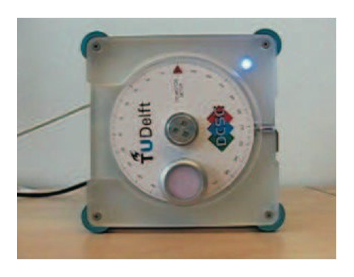
\includegraphics[width=.5\textwidth]{img/pendulum}
	\caption[Inverted pendulum setup]{Inverted pendulum setup.}
	\label{fig:PS-Inverted pendulum setup}
\end{figure}
The inverted pendulum was simulated in \textsc{Matlab} with a sampling time of \lsymb{$T_s$}{Sampling time}~$ = 0.03$~s. No noise was added to the system. The angle was wrapped to $\theta \in [-\pi, \pi]$ and the angular velocity was limited to $\omega \in [-10\pi, 10\pi]$. 
%A faster sampling time led to slower learning, a slower sampling time led to a worse resulting policy. 

\begin{table}[htbp]
	\centering
	\caption[Inverted pendulum: Parameter values]{Physical parameters of the inverted pendulum.}
	%                PAR.J = 0.005; PAR.K = 0.1; PAR.b = 0.01; PAR.m = 0.1; PAR.l = 0.1;
		\begin{tabular}{ll}
			\textbf{Symbol} & \textbf{Parameter} \\ \hline
			$m = 0.1 \textrm{ kg}$ & Pendulum mass \\
			$J = 1.91\cdot 10^{-4} \textrm{ kg/rad}^2$ & Pendulum inertia \\ %1.91E-4
			$g = 9.81 \textrm{ m/s}^2$ & Gravitational acceleration \\
			$l = 0.1 \textrm{ m}$ & Pendulum length \\
			$b = 0.01 \textrm{ kg/s}$ & Damping \\
			$K_R = 9.5 \Omega$ & Rotor resistance \\ %9.5
			$K_t = 5.36 \textrm{ Nm/A}$ & Torque constant %5.36E-4
		\end{tabular}
	\label{tab:PS-inverted pendulum parameters}
\end{table}


\subsection{Reward function}\label{sec:PS-learning problem reward}
The reward function can be implemented in two different ways. The first is a box-style reward. This reward originates from the idea that the goal state results in a reward and the other states in a penalty. As we are dealing with continuous states, we have to define a region around the goal that is considered close enough to the goal state. The box-style reward is defined as follows:
$$
	r(\theta,\omega) = 
		\left\{ \begin{array}{ll} 
%			+10, & \textrm{if } |\theta|<\delta_\theta \textrm{ and } |\omega|<\delta_\omega \\ 
			+10, & \textrm{if } |\theta|< \frac{10\pi}{180}\textrm{ rad} \textrm{ and } |\omega|< 0.3\textrm{ rad/s} \\  
			-1,  & \textrm{elsewhere} 
		\end{array} \right.
$$
%With $\delta_\theta$ and $\delta_\omega$ small values that define the region around zero that is considered to be the goal region. 
Where we have defined a region around zero that we consider as the goal region. With this type of reward, a learning trial is usually stopped when the goal region has been reached. 

Another option that is often used, is to use a smooth reward that gives a (negative) reward for every state-action pair:
$$
	\rho(\theta,\omega,u) = -\left[ \begin{array}{cc} \theta & \omega \end{array} \right]Q_\textrm{lq}\left[ \begin{array}{c} \theta \\ \omega \end{array} \right]- u R_\textrm{lq} u
$$
with $ Q_\textrm{lq} = \left[ \begin{array}{cc} 5 & 0 \\ 0 & 0.1 \end{array} \right]$ and $R_\textrm{lq} = 0.01$. This is a lqr-style reward and it will also drive the system to the goal state $[0, 0]^T$. Preliminary experiments showed that this reward resulted in a much faster learning speed than the box-reward, so we choose the smooth reward for the learning experiments. %\textcolor{red}{add: results box-style vs lqr-style}

A learning problem with lqr-rewards does not have an explicit goal state so learning trials are continuing. We have chosen to stop a trial whenever the goal region (as defined in the box-style reward) has been reached. This made no difference for the learning speed or the resulting policy. This can be explained by the fact that the system does not learn anything by moving around in the goal region. Adding a stopping criterion did reduce the simulation time significantly, since a large number of trials is stopped before maximum time for the episode ran out.

It has to be noted that although both reward structures have $[0, 0]^T$ as goal, the learning problem is not the same. The box-style reward results in a solution that gives the time-optimal policy to drive the system to the goal. The smooth reward results in a solution that is optimal with respect to the cost function $\rho$. This function also depends on the input signal $u$, so the optimal policy will try to limit the control signal as well as getting to the goal. The resulting policy will therefore not be time-optimal.



\subsection{Learning parameters}\label{sec:PS-learning problem parameters}
Tuning a \ac{RL} algorithm boils down to tuning three learning parameters: the discount factor $\gamma$, the learning rate $\alpha$ and the exploration rate $\epsilon$. The discount factor defines the solution to the learning problem and should therefore be fixed during the entire experiment. The learning rate influences how fast the value function is updated and thus how aggressively the agent learns. For noisy or stochastic experiments a high learning rate might lead to 'unlearning'. The exploration rate defines the percentage of random actions taken by the agent. The value may be constant or time-varying. The agent needs to explore in order to experience new state-action pairs and to avoid the learning of a sub-optimal policy. Unfortunately, no general rules for setting these parameters exist in the literature and the parameters have to be tuned empirically. 

We want to investigate the difference in performance between the \ac{RL} algorithms, we are not necessarily interested in the best performance for each case. Therefore, we did not try to fine-tune the parameters for every experiment, but set the tuning parameters to fixed values for all experiments. For \gsymb{$\gamma$}{Discount factor} and \gsymb{$\epsilon$}{Exploration rate} this seems reasonable. The first defines the solution and the second should have minor influence if multiple experiments are conducted. For the learning rate \gsymb{$\alpha$}{Learning rate} this might be questionable, because this factor immediately influences the update of the value function (\eqnref{eqn:RL-TDbasicQ}). The learning rate might have an optimal value for different experimental settings. For noisy environments or inaccurate models for instance, a low learning rate might be preferred. In noise-free environments with a very accurate model, a high learning rate might be used. Also different algorithms might have different optimal learning rates. 

The values of the learning parameters in a \ac{RL} experiment can be chosen freely and no rules for determining the optimal values exist. We chose the parameter values based on initial experiments and scientific intuition. The learning parameters were set as follows: 
$$
	\begin{aligned}
		\alpha &= 0.8 \\ 
		\gamma &= 0.98 \\
		\epsilon_{n_t} &= \max(0.1\cdot0.99^{n_t},0.001)
	\end{aligned}
$$
Where \lsymb{$n_t$}{Trial number} is the number of the current trial, so the exploration is decreased in every next trial, with a minimum of 0.001. A decreasing exploration rate led to faster learning than a fixed exploration rate and it led to a more 'smooth' learning curve. However, decreasing the exploration rate to zero led to occasionally finding a sub-optimal solution, so therefore the exploration was minimized to a small value. 


\subsection{Value function approximation: tile coding}\label{sec:PS-learning problem tile coding}
In the introduction of the value function in Section \ref{sec:RL-Value_functions}, it was assumed that a value is assigned to every state. This would lead to a tabular implementation of the value function in which every state has a value. As our state-space is continuous, this approach is impossible. Even discretizing the state-space into discrete bins, would still lead to a very large table. Therefore, we have to approximate the value function in some way.
\begin{figure}[htbp]
	\centering
		\includegraphics[width=.5\textwidth]{img/TileCoding}
%		\includegraphics[width=.5\textwidth]{img/Placeholder}
	\caption[Tile Coding]{Schematic overview of Tile Coding. The black dot represents a continuous value. The colored grids represent three tilings and the continuous value is approximated by the shaded tiles.}
	\label{fig:PS-TileCoding}
\end{figure}

Tile coding (\figref{fig:PS-TileCoding}) is a commonly used way to approximate functions, because it is fast and easy to use. We used tile coding as a function approximator for the action-value function. We used 20 tilings of $30\times 30$ tiles each, which led to a final resolution of approximately $\Delta_\theta=0.01$ for the angle $\theta$ and $\Delta_\omega=0.1$ for the angular velocity $\omega$. These values are exact only if the tilings are displaced evenly with respect to each other. Because we use random displacements, the given resolutions are approximations. The tiles were initialized with a random value in the interval $[0,1]$. Again, we are not interested in achieving the best performance for every algorithm, but in creating a fixed experimental setting for all experiments. It is expected that the value-function will only influence the quality of the final policy and not the difference between the policies of different algorithms. 

In all our experiments the actions available to the controller form a discrete set, so only a limited number of actions can be used. This is a common approach in \ac{RL} because it limits the number of state-action pairs. Hence the action-value function only has to generalize over the states and not over the actions.
%The actions were used as discrete inputs so no generalization over the actions was used.

%We used SARSA to perform value updates. Some quick experiments with Q-learning were conducted but they did not lead to significantly different results.



\section{Implementation of Local Linear Regression} \label{sec:PS-LLR implementation}
In this chapter we use two model-learning methods: Dyna and \ac{PS}. We use \ac{LLR} as a model to generate state-transitions in Dyna and to determine lead-in states in \ac{PS}. Prediction intervals are used as a possible accuracy measure of the modeled output. The number of nearest neighbors used in the linear regression will be fixed to $K=5$, a value that is based on the results with the two-link manipulator in Section \ref{sec:LLR-two link manipulator}. 
 
Every experiment started with an empty memory, which was updated with experienced state-transitions during the learning process. A $k$d-tree structure was used to represent the memory as described in Section \ref{sec:LLR-kd-tree}. New samples were added to the $k$d-tree immediately. In order to maintain a balanced tree, we re-built the entire tree after a learning trial was completed. After the first 1000 samples, the tree is not re-built between trials anymore and samples are added to the existing tree only. The main reason for this is that the re-building consumes too much time for many samples. Furthermore, the sample-density will be sufficiently high so that new samples will not unbalance the tree severely. The 1000-sample border is chosen more or less arbitrarily, based on experience gained with the \ac{LLR} experiments of Chapter \ref{chap:Modeling}. 




\subsection{Prediction intervals} \label{sec:PS-Prediction intervals}
It is expected that the accuracy of the \ac{LLR} model improves as the number of memory samples increases and that it can vary over the state-space. Our approach to assess the quality of the model is to use prediction intervals around the modeled state-transition (see Section \ref{sec:LLR-prediction interval}). 

We will introduce a limit on the prediction interval which has to guarantee accurate model outputs. The calculated prediction interval \lsymb{$I_x$}{Calculated prediction interval for variable $x$} will be compared to an user imposed limit \lsymb{$\delta_x$}{Imposed prediction interval limit for variable $x$}. Whenever the prediction interval is larger than the maximum value in any dimension, the modeled state-transition is discarded. We can write this mathematically as follows:
%For a prediction interval $I_{x_i}$ of the $i$th state $x_i$, we define the maximum prediction interval as $\delta_{x_i}$.
$$
	\hat{y}_q = 
	 	 \left\{\begin{array}{ll}
		 	\textrm{LLR}(x_q)  &, \quad \textrm{if $I_{x_i} \leq \delta_{x_i}$ for $i=1,2,\hdots,k$} \\
		 	\textrm{no answer} &, \quad \textrm{if $I_{x_i} > \delta_{x_i}$ for $i=1,2,\hdots,k$}  
		 \end{array}\right.
$$
If the prediction interval is smaller than this limit, the state-transition will be considered accurate enough to be used. If the prediction interval is larger, the estimated state-transition will be discarded and not used for learning. In our experiments a discarded estimation was not replaced by a different (possibly accurate enough) estimation. This replicates the real-time situation in which only a limited amount of time is available to estimate state-transitions. Endlessly calculating state-transitions until an accurate estimate is found, is therefore not possible.

As discussed earlier, we have no clear idea how small the interval has to be in order to indicate that the estimation is good enough to be used for \ac{RL}. The main problem is that we have no quantity to relate the interval to. That is, if this quantity exists at all. It might also be true that very inaccurate predictions can be used as long as they meet certain restrictions. These restrictions may vary, depending on the learning problem.
%For instance an estimated state-transition that points in the right direction, but with very inaccurate velocity, might still be used without disturbing the learning process.

At this point, we choose for the prediction interval a limit that is related to the final resolution of the value function approximator. The idea behind this choice is based on the discriminating power of the model and the value function approximator. It seems reasonable that the optimal situation is a value function approximator and a model that have about the same 'resolution'. Increasing the accuracy of only one of them, would only have a minor effect as the overall accuracy would be limited by the other. Computational resources are therefore used optimally if the model and the value function have a similar accuracy.  

We will use two prediction interval limits. The first is based in the tile size in each tiling. As we divide each tiling into $30\times 30$ tiles, the tile size is $\frac{2\pi}{30}\times \frac{20\pi}{30}$. The corresponding prediction interval limit is $[\delta_\theta, \delta_\omega]=[0.2094, 2.094]$. The second limit is based on the final resolution of the tile coding approximator. As we used 20 tilings, the approximate final resolution is $[\delta_\theta, \delta_\omega]=[\Delta_\theta,\Delta_\omega]=[0.01, 0.1]$. \figref{fig:TCvsPredInt} shows the prediction interval limit for a certain modeled state-transition.
%\gsymb{$[\delta_\theta, \delta_\omega]$}{full prediction interval}
\begin{figure}[htbp]
	\centering
		\includegraphics[width=.5\textwidth]{img/TCvsPREDINT}
	\caption[Prediction interval]{Limit of the prediction interval $[\delta_x,\delta_y]$ compared to the resolution of the value function $[\Delta_x,\Delta_y]$. The figure shows an estimated state-transition $s\rightarrow \hat{s}'$ with a prediction interval $[I_x,I_y]$. Because $[I_x,I_y]$ falls inside $[\delta_x,\delta_y]$, the corresponding prediction is considered accurate enough and is used for learning.}
	\label{fig:TCvsPredInt}
\end{figure}




\subsection{Lead-in states}\label{sec:PS-lead in states}

A crucial part in the \ac{PS} algorithm is determining lead-in states (Algorithm \ref{alg:PS}, line \ref{alg:PS_DetermineLeadInStates}). This process is not well described in literature. It is simply assumed that a model is available and that this model can be used to determine lead-in states. The type of model is not specified. We will describe our approach in this section.

First we have to note that we are actually not searching for lead-in states, but for lead-in state-action pairs. Consider the \ac{LLR} state-transition model \lsymb{$M$}{LLR model of the mapping $(s_t,a_t)\rightarrow s_{t+1}$} of the system. The state-transitions are then described by:
$$
	s_{t+1} = M \left[\begin{array}{c} s_t \\ a_t \\ 1 \end{array}\right]
$$
So we are actually searching for a state $s_t$ and an action $a_t$ that will lead to $s_{t+1}$. However, modeling the inverse mapping $s_{t+1}\rightarrow(s_t,a_t)$ would lead to two problems. First, one input could have several possible outputs (i.e., several state-action pairs $(s_t,a_t)$ can lead to $s_{t+1}$). So a unique model for this mapping does not exist. The second problem is that when this model would be used, we would obtain continuous values of $s_t$ and (more importantly) $a_t$. This is unwanted as we are assuming a discrete valued action-space.
%First, this mapping is ***Surjective?***. 

Our approach tries to solve these two issues. We consider the mapping $(s_{t+1},a_t)\rightarrow s_t$. This mapping can be modeled with an alternative model \lsymb{$\tilde{M}$}{LLR model of the mapping $(s_{t+1},a_t)\rightarrow s_t$} for which:
$$
	 s_t  = \tilde{M} \left[\begin{array}{c} s_{t+1} \\ a_t \\ 1 \end{array}\right]
$$
%Furthermore this mapping is ***injective??**, so the model is unique.
Because the action is now used as an input, we can choose a discrete value. The proposed mapping might seem counter intuitive, as the inputs are samples at different time steps. But this model should not be seen as an actual state-transition model. It should rather be regarded as a data mapping. We simply consider the sample $(s_{t+1}, a_t)$ as the input that leads to the output sample $s_t$. Note that the model $\tilde{M}$ is different from the state-transition model $M$. It is again obtained using \ac{LLR} techniques, but it requires a differently structured memory and a different input vector.

Now, for the target state $s$ the lead-in state-action pairs (\lsymb{$\bar{s}$}{Lead-in state to $s$},\lsymb{$\bar{a}$}{Lead-in action to $s$}) can be determined using the routine of Algorithm \ref{alg:lead-in states}. Note that every state, can have multiple lead-in states. Furthermore, we use the prediction interval limit (as described in Section \ref{sec:PS-Prediction intervals}) to possibly discard an estimated lead-in state. The notation $\bar{s}$ is used to denote a lead-in state to $s$. Subscripts containing time are usually avoided. 
\begin{algorithm}[ht]
	\caption{Lead-in states} \label{alg:lead-in states}
	\begin{algorithmic}[1]
		\State given $s$ 																\Comment{Target state}
		\For{ each $a \in \mathcal{A}$}
			\State $\tilde{M} \gets \textrm{LLR}(s,a)$ 		\Comment{Estimate LLR model $\tilde{M}$}
			\State $\hat{s} \gets \tilde{M}\left[\begin{array}{ccc} s & a & 1 \end{array}\right]^T$
			\If{ $I_{\hat{s}} \leq \delta_{s}$} 					\Comment{If prediction interval is sufficiently small}
				\State $(\bar{s},\bar{a})\gets(\hat{s},a)$ is a lead-in state	
			\EndIf		
		\EndFor
	\end{algorithmic}
\end{algorithm}


%\subsection{Look ahead Dyna (?)}
%\subsubsection{Estimating future states}






\section{Experimental results}\label{sec:PS-results}
We now present our experimental results. As explained in the beginning of this chapter, we used the same experimental setup and parameters for all experiments. All results shown in this section, are averages of 30 separate learning experiments. Every experiment consists of 1000 learning trials and every trial (or episode) consisted of a maximum of 100 time steps (equivalent to 3 seconds simulated time). This results in a maximum learning time of 50 minutes per experiment. Every experiment starts with a cleared \ac{LLR} memory and a randomly initialized value function.



\subsection{SARSA} \label{sec:PS-SARSA}
We have introduced the on-line, model-free algorithm SARSA in Section \ref{sec:RL-SARSA}. This is the most basic form of on-line learning. At every time step, one value function update is executed based on one real state-transition. SARSA can be considered as a 'benchmark' to which Dyna and \ac{PS} can be compared. In order for \ac{LLR} to be useful, the model-learning algorithms should perform better than a purely model-free algorithm. Furthermore, SARSA was used to get insight in the learning parameters and the optimal policy.

\figref{fig:PS-SARSA-learningcurve} shows the learning curve for the SARSA algorithm. The figure shows the reward per trial (a 3 second experiment), averaged over 30 separate experiments. We also show the standard deviation, minimum and maximum values in order to gain insight in the spread of the learning curve. The graph shows very rapid learning during the first 5~minutes. Thereafter, the policy strongly improves further until about 15~minutes of learning. The reason that the curve still fluctuates slightly thereafter is due to the exploration. 

Closer inspection of the experimental data, showed that it takes on average about 3~minutes to reach the goal for the first time. Although the maximum duration of a learning experiment is 50~minutes, the added stopping criterion leads to an average experiment length of 25.4~minutes. During this period the SARSA algorithm used on average $5.1\cdot 10^4$ real experiences to learn. 
\begin{figure}[htbp]
	\centering
	\subfigure[{SARSA learning curve}]{ 
		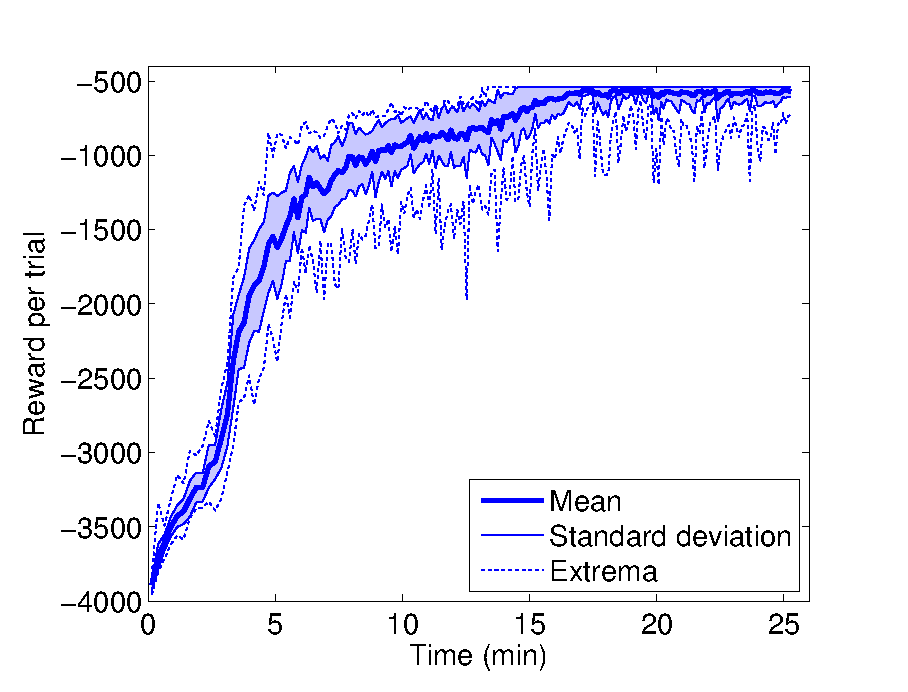
\includegraphics[width=.45\textwidth]{figures/PS-SARSA-learningcurve}	
	\label{fig:PS-SARSA-learningcurve}
	}
	\subfigure[{SARSA compared to Q-learning}]{ 
		\includegraphics[width=.45\textwidth]{figures/PS-SARSAvsQlearning}	
	\label{fig:PS-SARSAvsQlearning}
	}
%	\subfigure[{Optimal policy}]{ 
%		\includegraphics[width=.45\textwidth]{figures/PS-invpend_optimalpolicy}	
%	\label{fig:PS-optimal policy}
%	}
	\caption[Inverted pendulum: Model-free learning]{Learning curves of model-free learning applied on the inverted pendulum simulation. \subref{fig:PS-SARSA-learningcurve} shows the reward per trial during an experiment consisting of 1000 trials using SARSA as learning algorithm. The graph shows the average value (solid line), the standard deviation (shaded area) and the extreme values (dashed lines) of 30 separate experiments. \subref{fig:PS-SARSAvsQlearning} compares SARSA and Q-learning.}
	\label{fig:PS-SARSAlearningCurve}
\end{figure}

%In order to get insight in how the optimal policy looks, we executed a SARSA experiment for 10000 trials. \figref{fig:PS-optimal policy} shows the obtained %policy after 10000 trials. We use this policy as (an approximation of) the optimal policy for this problem.

We could also have used the model-free algorithm Q-learning (Section \ref{sec:RL-Q_learning}) instead of SARSA. Preliminary experiments with the two algorithms (\figref{fig:PS-SARSAvsQlearning}) showed no significant difference in learning speed between the two algorithms. When combined with function approximators, SARSA has better convergence properties than Q-learning \cite{Gordon:95}, so we will use SARSA to update the value function in the remaining of this chapter.
%\begin{figure}[htbp]
%	\centering
%		\includegraphics[width=.7\textwidth]{figures/PS-SARSAvsQlearning}
%	\caption[Inverted pendulum: SARSA compared to Q-learning]{Comparison of the learning curves using SARSA and Q-learning for the inverted pendulum. The graph compares the model-free SARSA (solid line) and Q-learning (dashed line) algorithms.}
%	\label{fig:PS-SARSAvsQlearning}
%\end{figure}

The learning curves presented in the chapter show the reward per trial. The results show that the agent learns a policy along the trajectory towards the goal. However, this does not necessarily mean that the policy has converged for the entire state-space. In Appendix \ref{app:Policies} we show the final policy for all learning algorithms and compares them to the optimal policy.

\subsection{Dyna} \label{sec:PS-Dyna}
We now add the \ac{LLR} model to the learning process and combine it with the Dyna algorithm (see Section \ref{sec:RL-Dyna}). The modeled state-action pairs are chosen randomly throughout the state-space. The \ac{LLR} model is built and used as described in Section \ref{sec:PS-LLR implementation}. Initially the memory is empty and every new experience is immediately added to it. We generated $N_m = 3$ state-transitions every time step. Prediction intervals of the \ac{LLR} model are used to possibly discard an estimate if it exceeds a given limit (see Section \ref{sec:PS-Prediction intervals}).

We compared several values for the maximum prediction interval. Due to the limit on the prediction interval, not all modeled state-transitions are used by the learning agent. \tabref{tab:PS-dyna updates} summarizes the number of iterations and value-function updates of the different settings. It is clear that setting this limit tighter, leads to more discarded model-outputs. In the case of a very tight limit of $[0.001,0.01]$, 86~\% of the modeled outputs get discarded. In the case of a less tight limit of $[0.2094,2.0944]$, only 37\% get discarded. 

\begin{table}[htbp]
	\centering
	\caption[Inverted pendulum: Learning results]{Results of the learning experiments on the inverted pendulum using different algorithms. The results are averages of 30 experiments, consisting of 1000 trials, generating $N_m=3$ modeled state-transitions per time interval. 'Iterations' are the total number of simulated time steps, 'Updates' are the total number of value-function updates (model-free and model-based), 'Ratio' is the ratio of model-free updates to model-based updates.}
		\begin{tabular}{l|llll}
			\textbf{Algorithm} & $[\delta_\theta,\delta_\omega]$ & \textbf{Iterations} $[10^4]$  & \textbf{Updates} [$10^4$]& \textbf{Ratio}  \\ 
			\hline\hline
			SARSA 								& -										&   4.95  &   4.95  & 1:0			\\  
			Q-learning 						&	-										&   5.11  &   5.11  & 1:0 		\\   
			\hline 
			Dyna 						  		& $[0.001, 0.01]$ 		&   4.94  &   6.98  & 1:0.41  \\ 
			(\ac{LLR} model)	 		& $[0.01, 0.1]$				&   4.22  &   8.73  & 1:1.07	\\ 
			 											& $[0.2094, 2.0944]$	&   3.97  &  11.93  & 1:2.01  \\ 
			 											& $[\infty,\infty]$		&   4.17  &  16.69  & 1:3     \\	
			\hline
			Dyna (exact model)		& -										&   3.65  &  14.61  & 1:3     \\
			\hline			 
			\acl{PS} 							& $[0.001, 0.01]$			&   4.77  &   9.30  & 1:0.95  \\ 
			(\ac{LLR} model) 			& $[0.01, 0.1]$				&   4.76  &  13.93  & 1:1.93  \\
			 											& $[0.2094, 2.0944]$	&   4.38  &  16.59  & 1:2.79  \\ 
			 											& $[\infty, \infty]$	&   6.31  &  25.24  & 1:3     
			\\ \hline
			Look Ahead Dyna				& $[0.001, 0.01]$			&   4.71  &  12.61  & 1:1.68	\\
			(\ac{LLR} model)			& $[0.01, 0.1]$				&   4.42  &  15.38  & 1:2.48	\\
														& $[0.2094, 2.0944]$	&   4.14  &  16.01  & 1:2.87 	\\
														& $[\infty, \infty]$	&   4.42  &  17.67  & 1:3      			 												
		\end{tabular}
	\label{tab:PS-dyna updates}
\end{table}
% Computation times (1000 trials/3000 seconds/50 minutes, Nm = 3, dualcore intel):
% SARSA: 	80 seconds/1.3 minutes	 --> 24 min experiment (~18x realtime)
% DYNA: 	170 seconds/~3 minutes   --> 20 min experiment (~6x realtime)
% LA: 		150	seconds/~2.5 minutes --> 20 min experiment (~8x realtime)
% PS: 		600 seconds/10 minutes   --> 22 min experiment (~2x realtime)

\begin{table}[htbp]
	\centering
	\caption[Computation times of the learning algorithms]{Computation time needed to perform all calculations in a single time step of the different learning algorithms for $N_m=3$. The table shows the mean time and the maximum time needed (during the entire experiment). The results were obtained using a 3~GHz desktop computer. Notice that the sampling time of the simulation is $T_s = 30\cdot 10^{-3}$~s.}
		\begin{tabular}{l|ll}
			\textbf{Algorithm} & \textbf{Mean [$10^{-3}$~s]} & \textbf{Max [$10^{-3}$~s]} \\ 
			\hline\hline
			SARSA & 1.01 & 1.94 \\
			Dyna  & 2.75 & 5.97 \\
			Prioritized Sweeping & 4.65 & 8.51 \\
			Look Ahead Dyna & 2.38 & 4.71 
		\end{tabular}
	\label{tab:PS-computation times}
\end{table}

%SARSA|   min: 0.00088196    max: 0.0019448    mean: 0.0010612
%DYNA|   min: 0.0019265    max: 0.0059695    mean: 0.0027438
%PS|   min: 0.00094839    max: 0.0085139    mean: 0.0046493
%LA|   min: 0.0010011    max: 0.0047052    mean: 0.0023847

We now continue with a closer inspection of the performance of the different \ac{LLR} settings. \figref{fig:PS-DYNA} shows the reward per trial during the learning process for the different settings. We notice that a large limit on the prediction interval leads to faster learning. The learning speed differs particularly in the first five minutes of the learning process. Furthermore, we notice that the spread in the learning curves increases with decreasing prediction interval limits. For very tight limits, the spread is very similar to the SARSA result. Using many uncertain outputs is preferred as this results in a smaller spread of the learning curve. This might be counter-intuitive as it is expected that highly inaccurate state-transitions lead to faulty value-function updates. However, this effect is apparently counteracted by the high number of value-function updates.

\begin{figure}[htbp]
	\centering
	\subfigure[{$[\delta_\theta,\delta_\omega]=[0.001,0.01]$}]{ 
		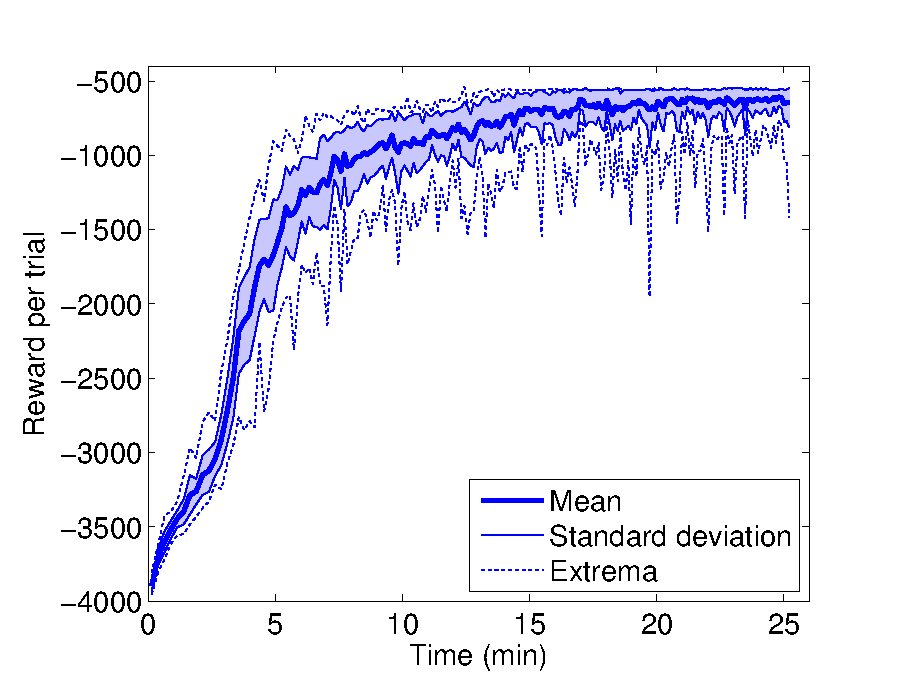
\includegraphics[width=.45\textwidth]{Figures/PS-DYNA1-learningcurve}
	\label{fig:PS-DYNA1-learningcurve}
	}
	\subfigure[{$[\delta_\theta,\delta_\omega]=[0.01,0.1]$}]{ 
		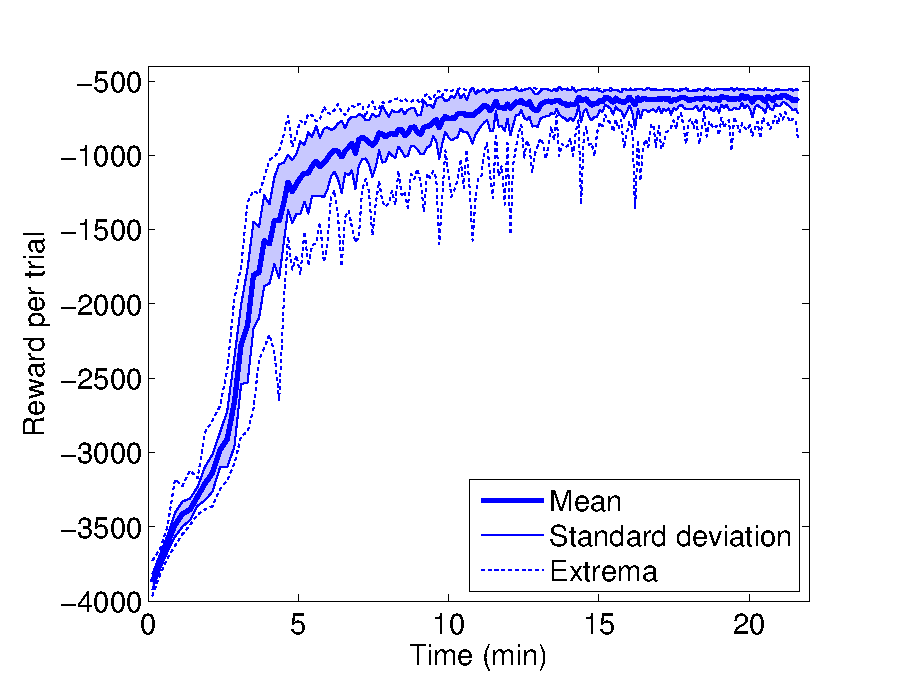
\includegraphics[width=.45\textwidth]{Figures/PS-DYNA2-learningcurve}
	\label{fig:PS-DYNA2-learningcurve}
	}\\
	\subfigure[{$[\delta_\theta,\delta_\omega]=[0.2094,2.0944]$}]{ 
		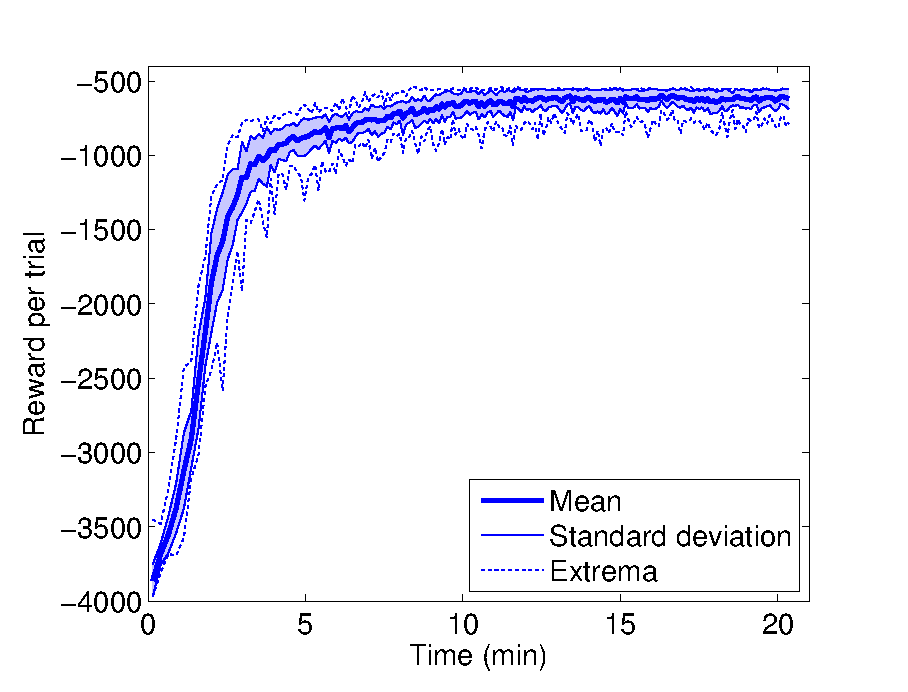
\includegraphics[width=.45\textwidth]{Figures/PS-DYNA3-learningcurve}
	\label{fig:PS-DYNA3-learningcurve}
	}
	\subfigure[{$[\delta_\theta,\delta_\omega]=[\infty,\infty]$}]{ 
		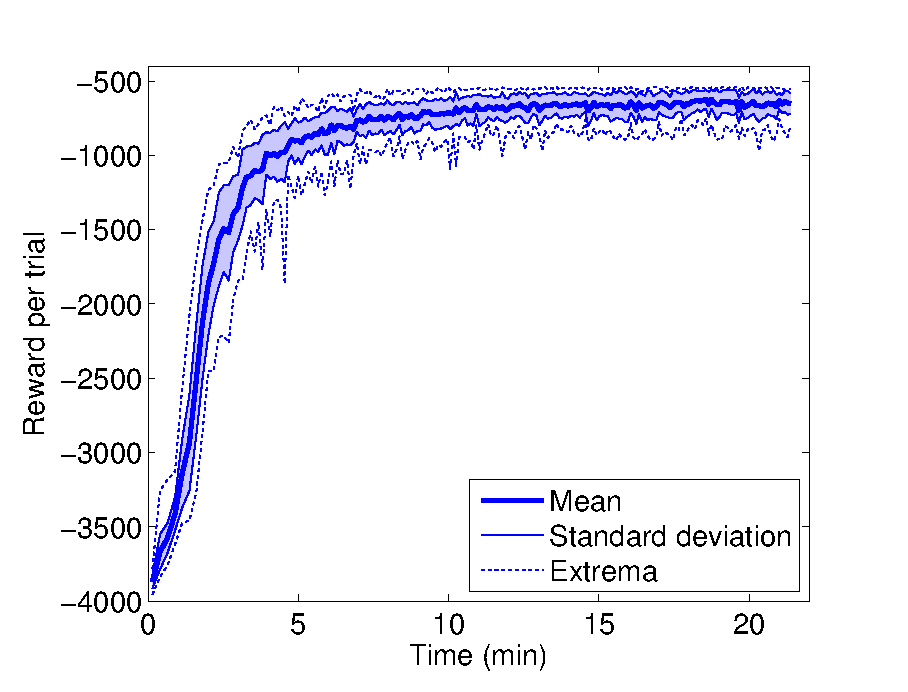
\includegraphics[width=.45\textwidth]{Figures/PS-DYNA4-learningcurve}
	\label{fig:PS-DYNA4-learningcurve}
	}
	\caption[Inverted pendulum: Dyna]{Learning curves of the Dyna algorithm applied on the inverted pendulum. \subref{fig:PS-DYNA1-learningcurve}, \subref{fig:PS-DYNA2-learningcurve}, \subref{fig:PS-DYNA3-learningcurve} and \subref{fig:PS-DYNA4-learningcurve} show the Dyna algorithm using \ac{LLR} with increasing prediction interval limits.}
	\label{fig:PS-DYNA}
\end{figure}

\figref{fig:PS-DYNA_hLLR} shows another effect of the limit on the prediction interval. The figure shows the positions in state-space for which a modeled state-transition was generated and not discarded. It is clear that the sample density and the prediction interval are related. For a very tight limit (\figref{fig:PS-DYNA1_hLLR}), only in the vicinity of the optimal trajectory enough samples are available for an estimated state-transition that is accurate enough. When the limit is stretched (\figref{fig:PS-DYNA2_hLLR}-\ref{fig:PS-DYNA3_hLLR}), so is the region in which the model is considered to be accurate enough. If no limit is imposed (\figref{fig:PS-DYNA4_hLLR}), the modeled state-transitions in the entire state-space are used.

\begin{figure}[htbp]
	\centering
	\subfigure[{$[\delta_\theta,\delta_\omega]=[0.001,0.01]$}]{
		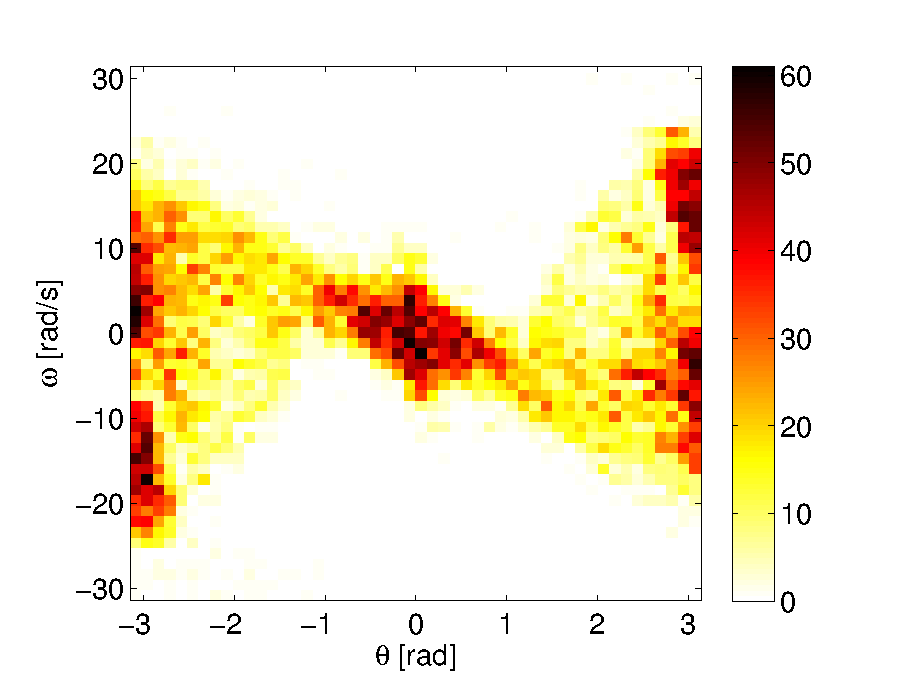
\includegraphics[width=.45\textwidth]{Figures/PS-DYNA1_hLLR}
	\label{fig:PS-DYNA1_hLLR}
	}
	\subfigure[{$[\delta_\theta,\delta_\omega]=[0.01,0.1]$}]{ 
		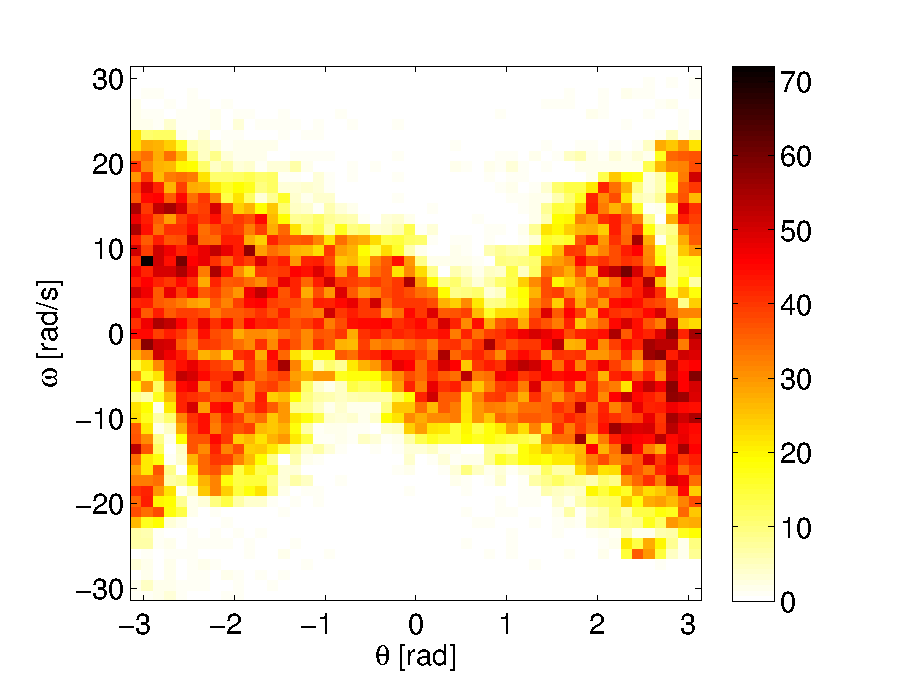
\includegraphics[width=.45\textwidth]{Figures/PS-DYNA2_hLLR}
	\label{fig:PS-DYNA2_hLLR}
	}\\
	\subfigure[{$[\delta_\theta,\delta_\omega]=[0.2094,2.0944]$}]{
		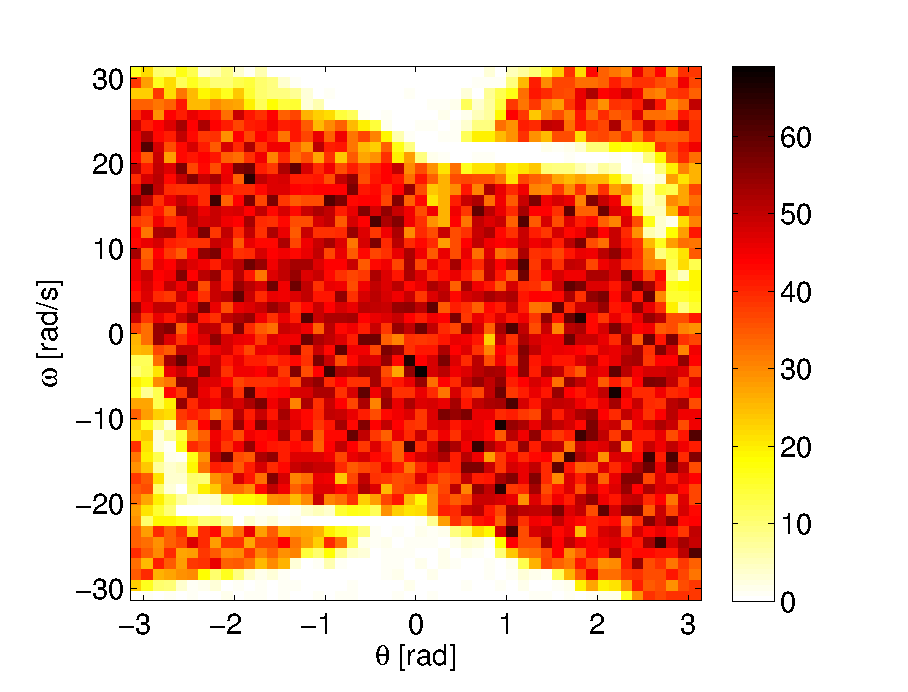
\includegraphics[width=.45\textwidth]{Figures/PS-DYNA3_hLLR}
	\label{fig:PS-DYNA3_hLLR}
	}
	\subfigure[{$[\delta_\theta,\delta_\omega]=[\infty,\infty]$}]{
		\includegraphics[width=.45\textwidth]{Figures/PS-DYNA4_hLLR}
	\label{fig:PS-DYNA4_hLLR}
	} 
	\caption[Inverted pendulum: Distribution of model-generated experience using Dyna]{Distribution of states for which a state-transition was generated using the \ac{LLR} model in the Dyna setting. The figures only show the states for which the prediction interval was smaller than the given limit. The color indicates the number of times a state-transition was generated in a certain area.}
	\label{fig:PS-DYNA_hLLR}
\end{figure}

\figref{fig:PS-SARSAvsDYNA} shows the average learning curve of the Dyna algorithms compared to model-free SARSA learning. We conclude that using model-generated experience in the learning process increases the learning speed. Increasing the limit on the prediction interval leads to more state-transition available to the agent. The graph shows that this leads to faster learning. The inaccuracy of these state-transition does not seem to influence the learning process negatively. 

Although all algorithms converge, the final reward per trial is slightly higher for SARSA. This indicates that the final trajectory towards the goal for SARSA is slightly better, with respect to the reward function, than for Dyna. So we can conclude that adding state-transitions generated by the \ac{LLR} model only has a minor negative effect on the resulting trajectory, even if highly inaccurate state-transitions are being used. Apparently, the number of real experience and accurate modeled state-transitions are high enough to counteract the negative effect of the inaccurate model outputs. Furthermore, it can be expected that the inaccurate state-transitions can mainly be found in rarely visited parts of the state-space (see also \figref{fig:PS-DYNA_hLLR}). These regions have a limited effect on the trajectory towards to goal.

A question posed earlier was: is it more useful to use many inaccurate model-outputs or to use a limited number of very accurate outputs? If we regard the prediction interval as a good indication, we can answer this question by comparing the values in \tabref{tab:PS-dyna updates} with the learning curves in \figref{fig:PS-SARSAvsDYNA}. It can be concluded that the number of value-function updates is dominant over the quality of the state-transitions. In other words, the optimal setting for Dyna in this test setup is to use as many model-outputs as possible by setting the limit on the prediction interval to a high value.
\begin{figure}[htbp]
	\centering
		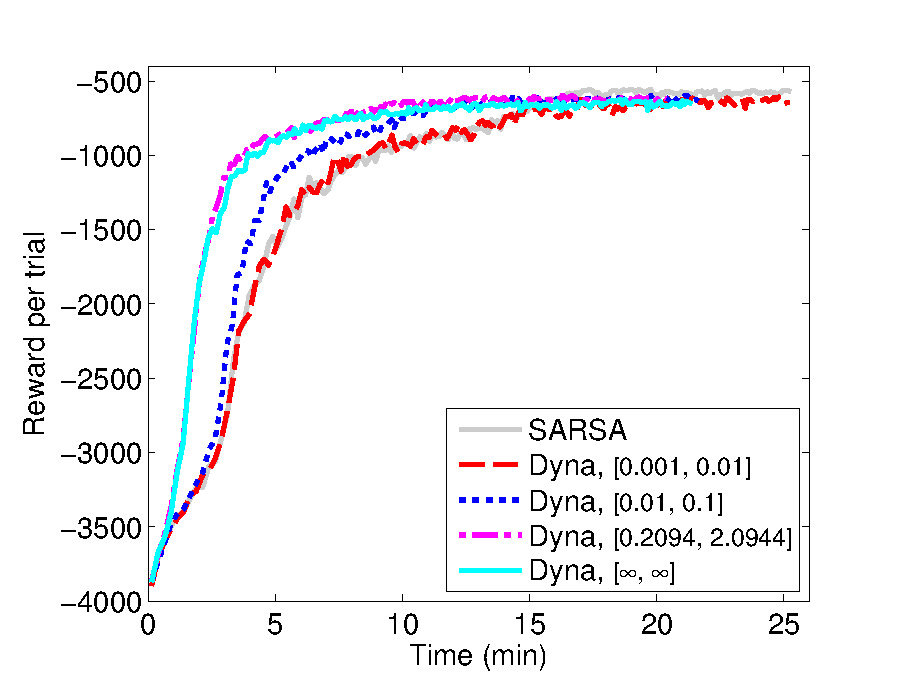
\includegraphics[width=.7\textwidth]{figures/PS-SARSAvsDYNA}
	\caption[Inverted pendulum: Dyna compared to SARSA]{Comparison of the learning curves using SARSA and Dyna for the inverted pendulum for several values of the prediction interval limit $[\delta_\theta,\delta_\omega]$.}
	\label{fig:PS-SARSAvsDYNA}
\end{figure}

From the results in this section we can conclude that generating state-transitions using the \ac{LLR} model can increase the learning speed compared to model-free SARSA. We have seen that limiting the prediction interval influences the learning speed. However, we do not have an indication of the accuracy of the modeled state-transitions. For this, we need the true state-transitions. These can be obtained from \eqnref{eqn:PS-inverted pendulum}. We have applied Dyna using the exact model. This represents the optimal Dyna setting: a perfect model of the system throughout the state-space. We define the prediction interval of the exact model as $I = [0, 0]$. In \figref{fig:PS-DYNA4vsDYNANL} we compared the exact model to the optimal \ac{LLR} model. 

We notice that the curves are very close together. This means that the \ac{LLR} model does not disturb the learning process compared to the true model. In the first minutes of learning, both methods perform almost equally. This is surprising, as it is expected that early in the learning process the \ac{LLR} is not very accurate yet because of the low number of memory samples. Apparently, possibly inaccurate model outputs are still suitable for learning in the beginning. In the remaining of the learning process, the exact model has a very slight advantage over the \ac{LLR} model. 

The inaccuracy of the \ac{LLR} model is best seen in the later stages of the learning process. Although both learning curves converge to more or less the same value, the standard deviation of the exact model is about half the size of the \ac{LLR} model. This is caused by the inaccurate model outputs that are used by the Dyna algorithm using the \ac{LLR} model. 

\begin{figure}[htbp]
	\centering
		\includegraphics[width=.7\textwidth]{figures/PS-DYNA3vsDYNANL}
	\caption[Inverted pendulum: Dyna, \acs{LLR} model compared to exact model]{Comparison of the learning curves using Dyna with the \ac{LLR} model and the exact model on the inverted pendulum. We used $[\delta_\theta,\delta_\omega]=[0.2094, 2.0944]$ for the prediction interval limit of the \ac{LLR} model, which is the optimal setting.}
	\label{fig:PS-DYNA4vsDYNANL}
\end{figure}

In Section \ref{sec:LLR-kd-tree} we explained how we used a $k$d-tree to represent the memory in order to increase the computational speed of the \ac{LLR} model. Although in these simulation experiments the computation time is not limited, in real-time experiments all the calculations need to be performed within the sampling interval. The sampling time of the simulation was set to $T_s = 0.03$~s. Table \ref{tab:PS-computation times} shows the time needed by the learning algorithms in every sampling interval to perform all the calculations. The exact computation times will depend on the hardware and software used, so the values should be regarded only as indicative.

\subsection{Prioritized Sweeping}
We continue with \ac{PS} as a learning algorithm. Our \ac{PS} implementation will combine \ac{PS} (Algorithm \ref{alg:Dyna}) with \ac{LLR}. The lead-in states will be calculated as described in Section \ref{sec:PS-lead in states} and we set limits on the prediction interval in the same way as we did for Dyna. 
%The prediction interval limits are also used in determining the lead-in states (Algorithm \ref{alg:lead in states}).

First we investigate the influence of the prediction interval limit. \figref{fig:PS-PS} shows the learning curves for the \ac{PS} algorithm for several limits. We notice that the results differ in many aspects from the Dyna results. First we notice that for \ac{PS} we find an optimal value for the prediction interval limit. Out of the four intervals we have compared, $[\delta_\theta,\delta_\omega]=[0.2094,2.0944]$ performs best. This limit performs best both in terms of learning speed and in the variance of the learning curves. The other interval limits lead to worse results, with the worst result for $[\infty, \infty]$. For this large limit, the learning curve shows very slow learning, a large spread and no convergence to the optimal policy. Apparently the number of inaccurate state-transitions is so large that they severely disturb the learning process.

\begin{figure}[htbp]
	\centering
	\subfigure[{$[\delta_\theta,\delta_\omega]=[0.001,0.01]$}]{
		\includegraphics[width=.45\textwidth]{Figures/PS-PS1-learningcurve}
	\label{fig:PS-PS1-learningcurve}
	}
	\subfigure[{$[\delta_\theta,\delta_\omega]=[0.01,0.1]$}]{ % $0.001, 0.01$]{ %
		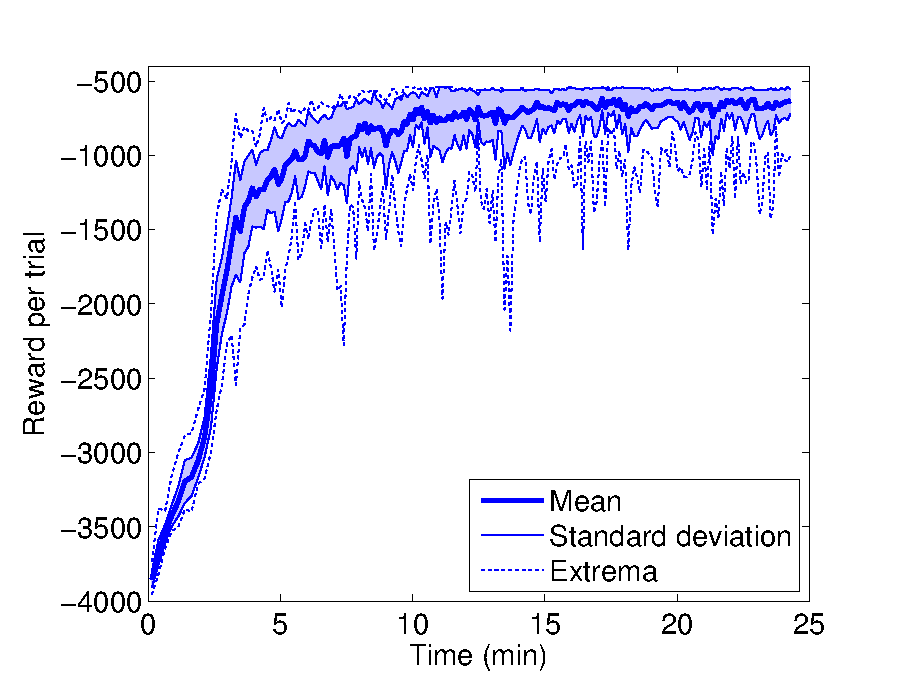
\includegraphics[width=.45\textwidth]{Figures/PS-PS2-learningcurve}
	\label{fig:PS-PS2-learningcurve}
	}\\
	\subfigure[{$[\delta_\theta,\delta_\omega]=[0.2094,2.0944]$}]{
		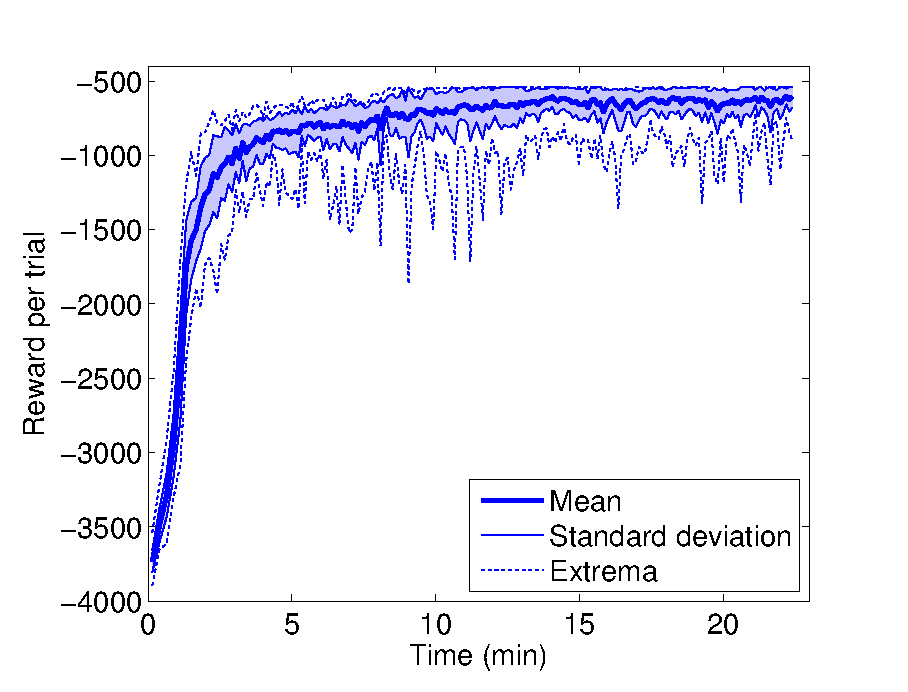
\includegraphics[width=.45\textwidth]{Figures/PS-PS3-learningcurve}
	\label{fig:PS-PS3-learningcurve}
	}
	\subfigure[{$[\delta_\theta,\delta_\omega]=[\infty,\infty]$}]{
		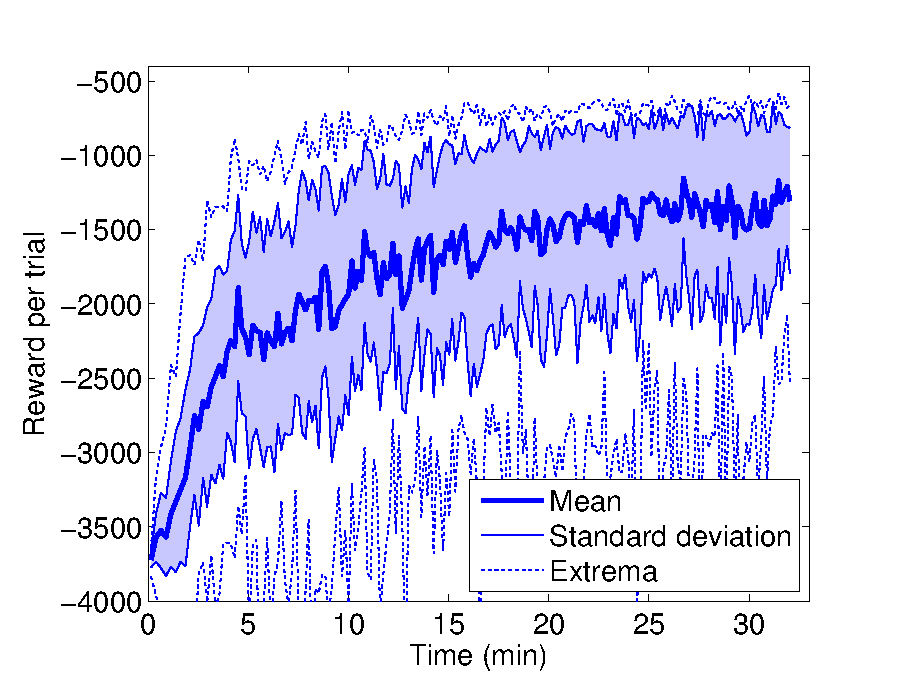
\includegraphics[width=.45\textwidth]{Figures/PS-PS4-learningcurve}
	\label{fig:PS-PS4-learningcurve}
	} 
	\caption[Inverted pendulum: \acs{PS}]{Learning curves of \ac{PS} applied on the inverted pendulum problem. \subref{fig:PS-PS1-learningcurve}, \subref{fig:PS-PS2-learningcurve}, \subref{fig:PS-PS3-learningcurve} and \subref{fig:PS-PS4-learningcurve} show the \ac{PS} algorithm using \ac{LLR} with increasing prediction interval limits.}
	\label{fig:PS-PS}
\end{figure}

\begin{figure}[htbp]
	\centering
	\subfigure[\ac{PS} learning curves]{ 
		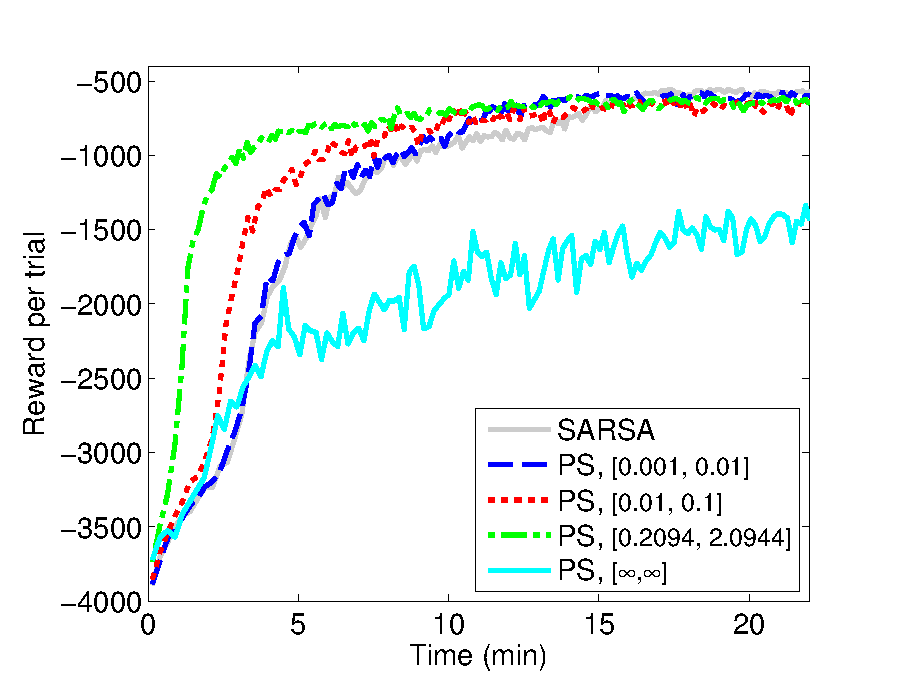
\includegraphics[width=.45\textwidth]{Figures/PS-PSlearningcurves}
	\label{fig:PS-PSlearningcurves}
	}	
	\subfigure[Comparison of \ac{PS}, Dyna and SARSA]{
		\includegraphics[width=.45\textwidth]{Figures/PS-PSvsDYNAvsSARSA}
	\label{fig:PS-PSvsDYNAvsSARSA}
	}
	\caption[Inverted pendulum: \acs{PS} compared to Dyna and SARSA]{Learning curves for \ac{PS} algorithm applied on the inverted pendulum setup. \subref{fig:PS-PSlearningcurves} compares \ac{PS} using four different values for the prediction interval limit, \subref{fig:PS-PSvsDYNAvsSARSA} compares the optimal settings of \ac{PS}, Dyna and SARSA.}
	\label{fig:PS-PScompared}
\end{figure}

\figref{fig:PS-PSlearningcurves} compares the learning speed of the different \ac{PS} settings. It is clear that \ac{PS} needs a limit on the prediction interval. The setting with no limit leads to a very slow learning speed, even slower than SARSA. In the 1000-trial experiment, this setting did not converge to a solution. Also the setting with very tight bounds does not perform well. This setting leads to a learning speed that is similar to model-free SARSA.

%\begin{figure}[htbp]
%	\centering
%		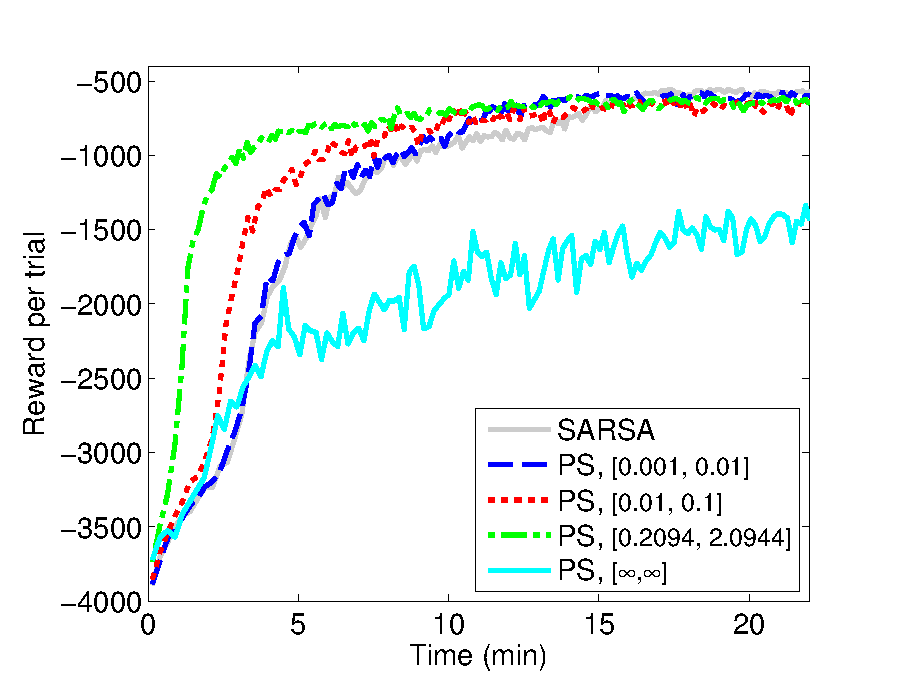
\includegraphics[width=.7\textwidth]{figures/PS-PSlearningcurves}
%	\caption[Inverted pendulum: Prioritized Sweeping compared to SARSA]{Learning curves of \ac{PS} compared to SARSA for the inverted pendulum. Several values for the prediction interval limit $[\delta_\theta,\delta_\omega]$ are shown.}
%	\label{fig:PS-PSlearningcurves}
%\end{figure}

%\begin{figure}[htbp]
%	\centering
%		\includegraphics[width=.7\textwidth]{figures/PS-PSvsDynavsSarsa}
%	\caption[Inverted pendulum: Prioritized Sweeping, Dyna and SARSA compared]{Learning curves of SARSA, Dyna and \ac{PS}. For all algorithms the setting with the best result is shown. Dyna: $[0.2094,2.0944]$, \ac{PS}: $[0.2094,2.0944]$.}
%	\label{fig:PS-PSvsDynavsSarsa}
%\end{figure}

It is also interesting to look at the number of updates used by the best ($[0.2094,2.0944]$) and worst ($[\infty,\infty]$) \ac{PS} case (\tabref{tab:PS-dyna updates}). We notice that the ratio's of the optimal (1:2.79) and worst (1:3) setting are actually very close together. Hence, the number of discarded state-transitions in the optimal case is not much higher. But apparently, the small amount of inaccurate estimates is enough to severely influence the learning process negatively.

If we compare the ratio of the model-generated versus model-free state-transitions of Dyna and \ac{PS} we notice that this ratio is higher in \ac{PS}. The priority queue leads to generated state-transitions that are close to the trajectory to the goal state. In these areas the number of memory samples is high and therefore accurate predictions can be made. Therefore, less model outputs are rejected than in the Dyna case where state-transitions are generated randomly in the entire state-space.

The best performance is obtained with the interval limit $[0.2094,2.0944]$. \figref{fig:PS-PSvsDYNAvsSARSA} shows the learning curve of the optimal \ac{PS} algorithm compared to Dyna and SARSA. The figure shows that the \ac{PS} algorithm learns faster than both Dyna and SARSA. Especially in the first minutes of learning, the prioritized updates of the value-function lead to faster learning than Dyna.



%\begin{figure}[htbp]
%	\centering
%	\subfigure[{$[\delta_\theta,\delta_\omega]=[0.001,0.01]$}]{
%		\includegraphics[width=.45\textwidth]{Figures/PS-PS1_hLLR}
%	\label{fig:PS-PS1_hLLR}
%	}
%	\subfigure[{$[\delta_\theta,\delta_\omega]=[0.01,0.1]$}]{ 
%		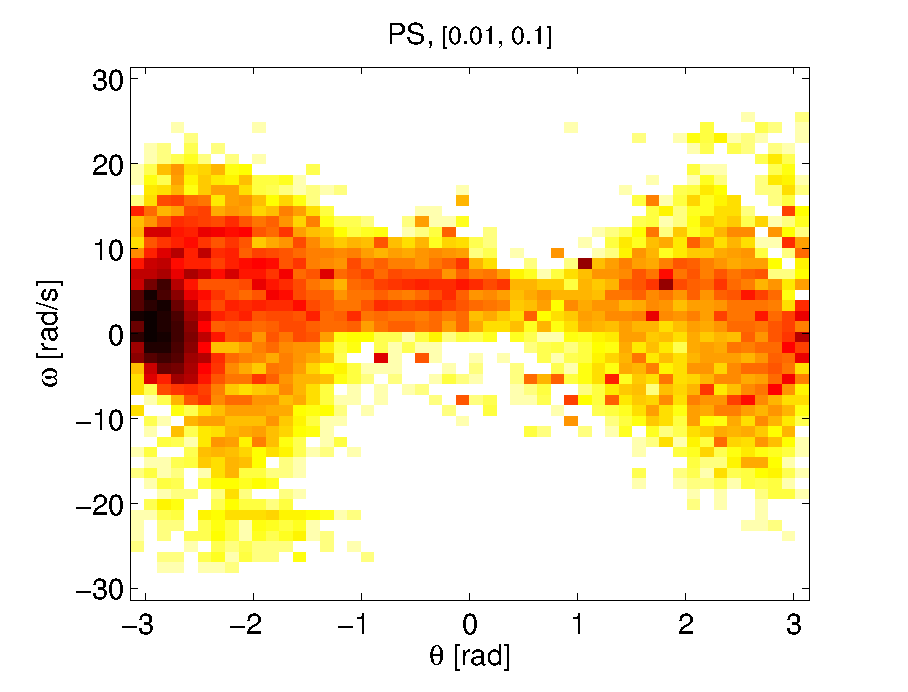
\includegraphics[width=.45\textwidth]{Figures/PS-PS2_hLLR}
%	\label{fig:PS-PS2_hLLR}
%	}\\
%	\subfigure[{$[\delta_\theta,\delta_\omega]=[0.2094,2.0944]$}]{
%		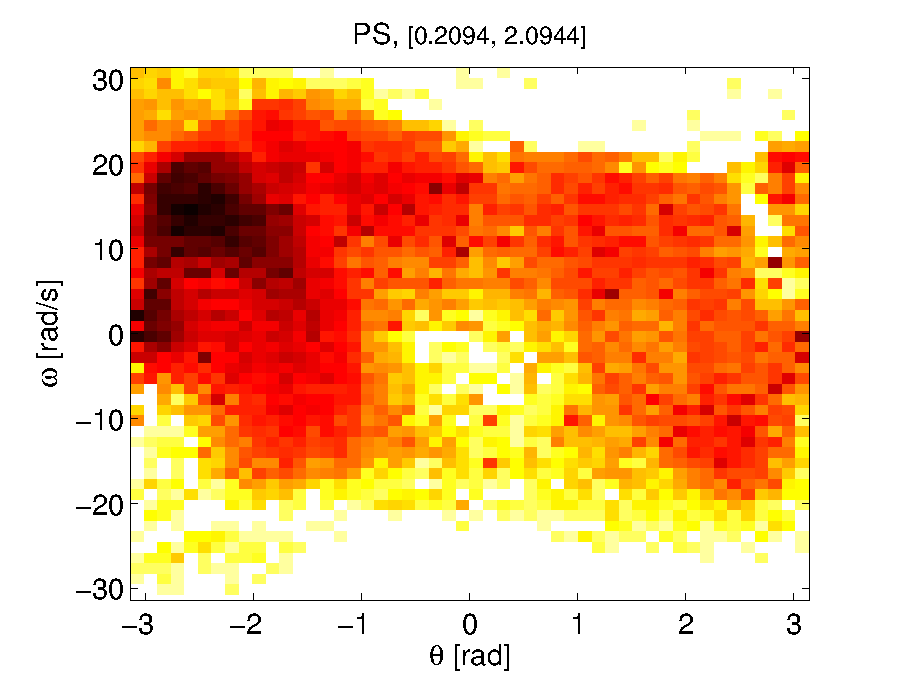
\includegraphics[width=.45\textwidth]{Figures/PS-PS3_hLLR}
%	\label{fig:PS-PS3_hLLR}
%	}
%	\subfigure[{$[\delta_\theta,\delta_\omega]=[\infty,\infty]$}]{
%		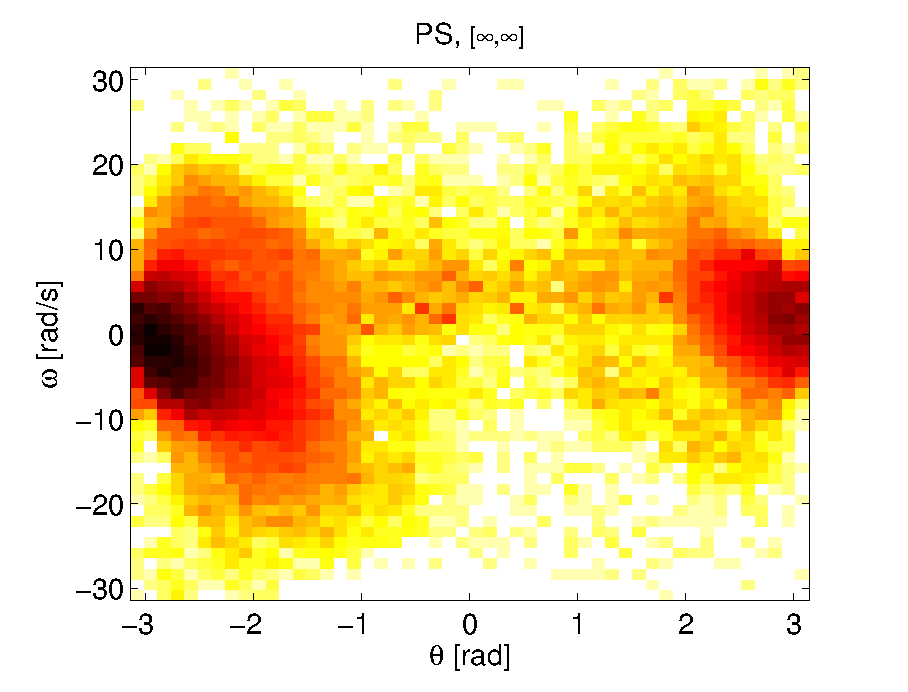
\includegraphics[width=.45\textwidth]{Figures/PS-PS4_hLLR}
%	\label{fig:PS-PS4_hLLR}
%	} 
%	\caption[Inverted pendulum: Sample distribution]{Distribution of states for which a modeled state-transitions was generated in the Dyna setting. The figures only show the states for which the prediction interval was smaller than the given limit.}
%	\label{fig:PS-PS_hLLR}
%\end{figure}

\subsection{Look Ahead Dyna} 
Let us consider \ac{PS} simply as a method to generate specific model-based experiences instead of random experiences. We then might introduce other methods to generate useful state-transitions - not necessarily according to a priority measure. A possible method could be to use the model to 'look ahead' from the current state. Imagine a state-transition $s \rightarrow s'$. We then use the model to estimate $s' \rightarrow s''$ for all actions. The only issue is that the next state $s'$ is not yet known when the model-based experiences are generated. Therefore, the next state has also got to be estimated. Algorithm \ref{alg:Look Ahead Dyna} shows this method, which we will call \ac{LA Dyna}.

The Look Ahead approach partly originates from the earlier \ac{LLR} experiments on the two-link manipulator and robot Leo (Sections \ref{sec:LLR-two link manipulator} and \ref{sec:LLR-robot leo}). In those settings we used the \ac{LLR} model to estimate a state-transition in the vicinity of the current state. \ac{LLR} was able to generate very accurate estimates of complex systems using only a small number of experiences. We use this ability to model future state-transitions in this 'Look Ahead' setting.
\begin{algorithm}[ht]
	\caption{Look Ahead Dyna} \label{alg:Look Ahead Dyna}
	\begin{algorithmic}[1]
		\State Initialize $Q(s,a)$ randomly
		\For{ each time step $t$}
			\State $s\gets \textrm{ Current state}$
			\State Select $a$ using policy
			\State Execute $a$ 
			\State Estimate $\hat{s}' \gets \textrm{LLR }(s,a)$
			\For{each $a\in \mathcal{A}$}
				\State $(\hat{s}'',r) \gets Model(\hat{s}',a)$
				\State $\delta \gets r + \gamma Q(\hat{s}'',a') - Q(\hat{s}',a)$
				\State $Q(s',a) \gets Q(s',a) + \alpha \delta$
			\EndFor
			\State Observe $s'$, $r$
			\State $\delta \gets r + \gamma Q(s',a') - Q(s,a)$
			\State $Q(s,a) \gets Q(s,a) + \alpha \delta$
		\EndFor
	\end{algorithmic}
\end{algorithm}


\subsubsection{Results}
We applied \ac{LA Dyna} on the inverted pendulum simulation. \figref{fig:PS-LA} shows the resulting learning curves for different values of the prediction interval limit. The prediction interval is needed in the \ac{LA Dyna} algorithm. No limit on the prediction interval leads to severe 'unlearning', as can be seen in \figref{fig:PS-LA4-learningcurve}. This effect was also seen in the case of the \ac{PS} algorithm. Clearly, when the value function updates are close to the optimal trajectory, the estimated state-transitions need to be accurate. 

\begin{figure}[htbp]
	\centering
	\subfigure[{$[\delta_\theta,\delta_\omega]=[0.001,0.01]$}]{ 
		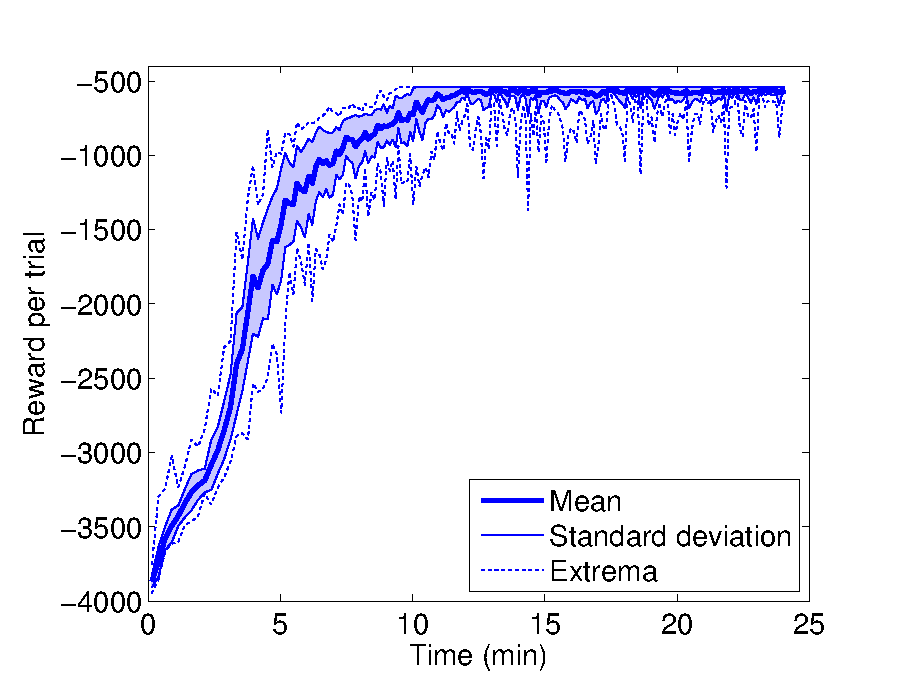
\includegraphics[width=.45\textwidth]{Figures/PS-LA1-learningcurve}
	\label{fig:PS-LA1-learningcurve}
	}
	\subfigure[{$[\delta_\theta,\delta_\omega]=[0.01,0.1]$}]{ 
		\includegraphics[width=.45\textwidth]{Figures/PS-LA2-learningcurve}
	\label{fig:PS-LA2-learningcurve}
	}\\
	\subfigure[{$[\delta_\theta,\delta_\omega]=[0.2094,2.0944]$}]{ 
		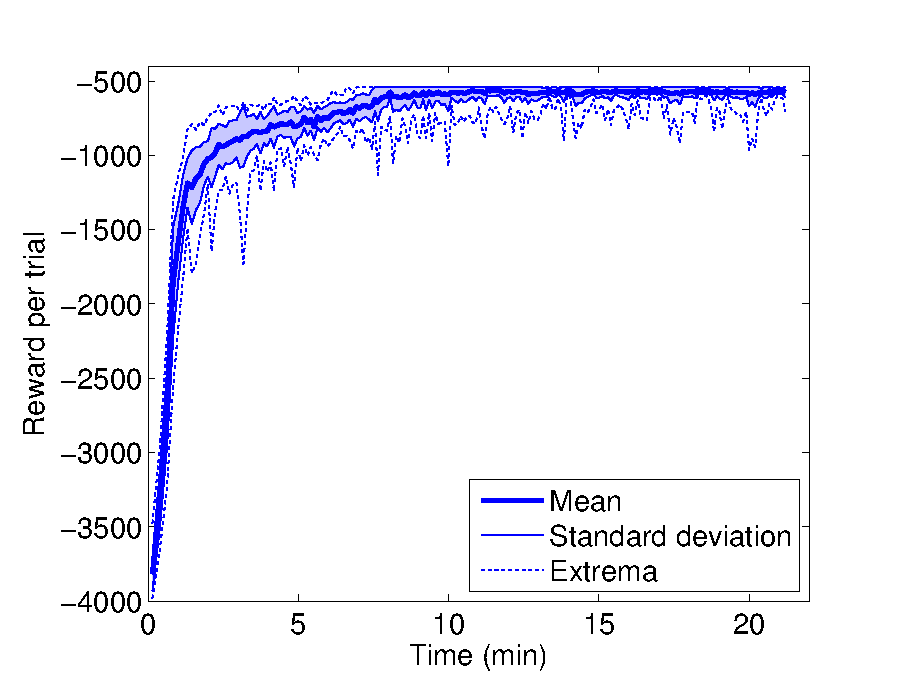
\includegraphics[width=.45\textwidth]{Figures/PS-LA3-learningcurve}
	\label{fig:PS-LA3-learningcurve}
	}
	\subfigure[{$[\delta_\theta,\delta_\omega]=[\infty,\infty]$}]{ 
		\includegraphics[width=.45\textwidth]{Figures/PS-LA4-learningcurve}
	\label{fig:PS-LA4-learningcurve}
	}
	\caption[Inverted pendulum: \acs{LA Dyna}]{Learning curves of the \ac{LA Dyna} algorithm applied on the inverted pendulum. \subref{fig:PS-LA1-learningcurve}, \subref{fig:PS-LA2-learningcurve}, \subref{fig:PS-LA3-learningcurve} and \subref{fig:PS-LA4-learningcurve} show the \ac{LA Dyna} algorithm using \ac{LLR} with increasing prediction interval limits.}
	\label{fig:PS-LA}
\end{figure}

\begin{figure}[htbp]
	\centering
	\subfigure[\ac{LA Dyna} learning curves]{ 
		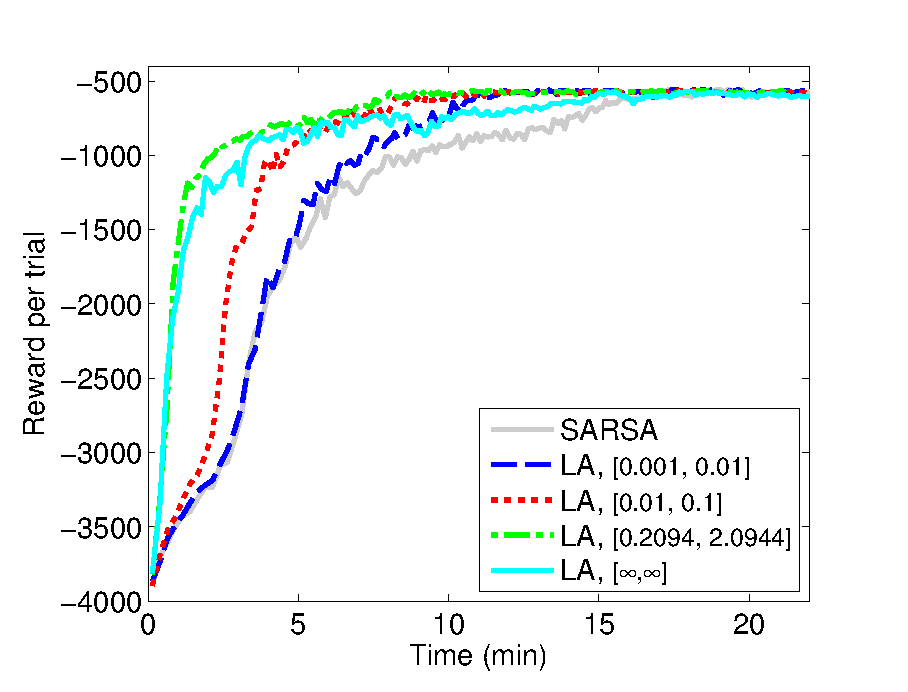
\includegraphics[width=.45\textwidth]{Figures/PS-LAlearningcurves}
	\label{fig:PS-LAlearningcurves}
	}	
	\subfigure[Comparison of \ac{LA Dyna}, \ac{PS}, Dyna and SARSA]{
		\includegraphics[width=.45\textwidth]{Figures/PS-LAvsPSvsDYNAvsSARSA}
	\label{fig:PS-LAvsPSvsDYNAvsSARSA}
	}
	\caption[Inverted pendulum: \acs{LA Dyna} compared to \acs{PS}, Dyna and SARSA]{Learning curves for the \ac{LA Dyna} algorithm applied on the the inverted pendulum setup. \subref{fig:PS-LAlearningcurves} compares \ac{LA Dyna} using four different values for the prediction interval limit, \subref{fig:PS-LAvsPSvsDYNAvsSARSA} compares the optimal settings of the four different learning algorithms.}
	\label{fig:PS-LAcompared}
\end{figure}

The optimal value for the prediction interval limit is $[0.2094,2.0944]$, which is equal to the optimal value for Dyna and \ac{PS}.

In \figref{fig:PS-LAvsPSvsDYNAvsSARSA} we compared \ac{LA Dyna} to SARSA, Dyna and \ac{PS}. It can be seen that \ac{LA Dyna} learns faster than the other algorithms. The faster learning can mainly be seen in the first part of the learning process. The \ac{LA Dyna} algorithm also results in less spread in the learning speed. The variance of the \ac{LA Dyna} is about half of the variance of the other algorithms.

\figref{fig:PS-LA_hLLR} shows the distribution of the model-generated state-transitions. As expected, the state-transitions are located primarily in the neighborhood of the trajectories followed by the system. A possible reason for the fast learning of \ac{LA Dyna} could be that the majority of the value function updates are very close to the current state of the real system.

\begin{figure}[htbp]
	\centering
	\subfigure[{$[\delta_\theta,\delta_\omega]=[0.001,0.01]$}]{
		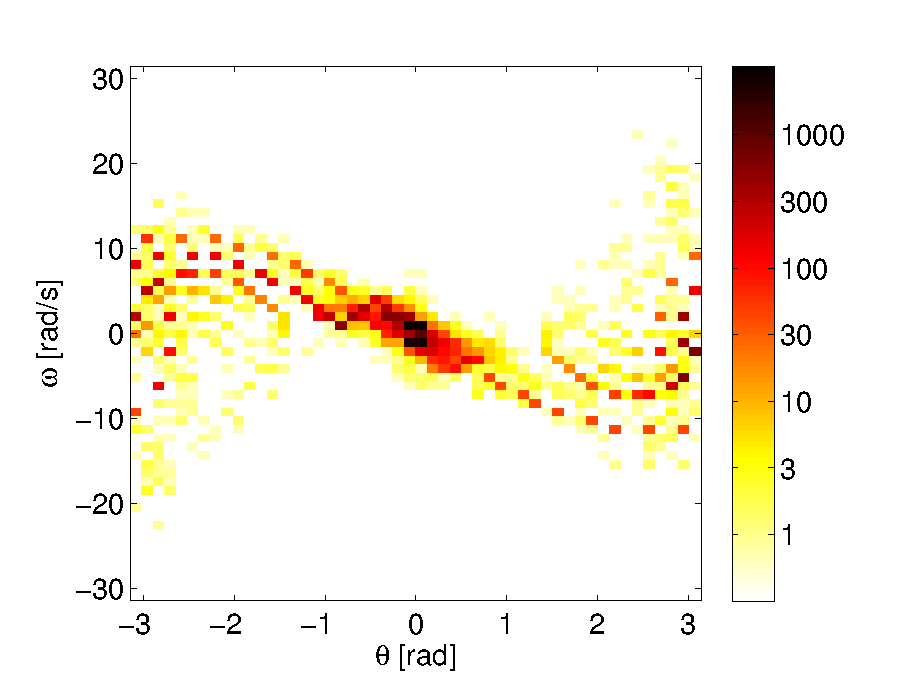
\includegraphics[width=.45\textwidth]{Figures/PS-LA1_hLLR}
	\label{fig:PS-LA1_hLLR}
	}
	\subfigure[{$[\delta_\theta,\delta_\omega]=[0.01,0.1]$}]{ 
		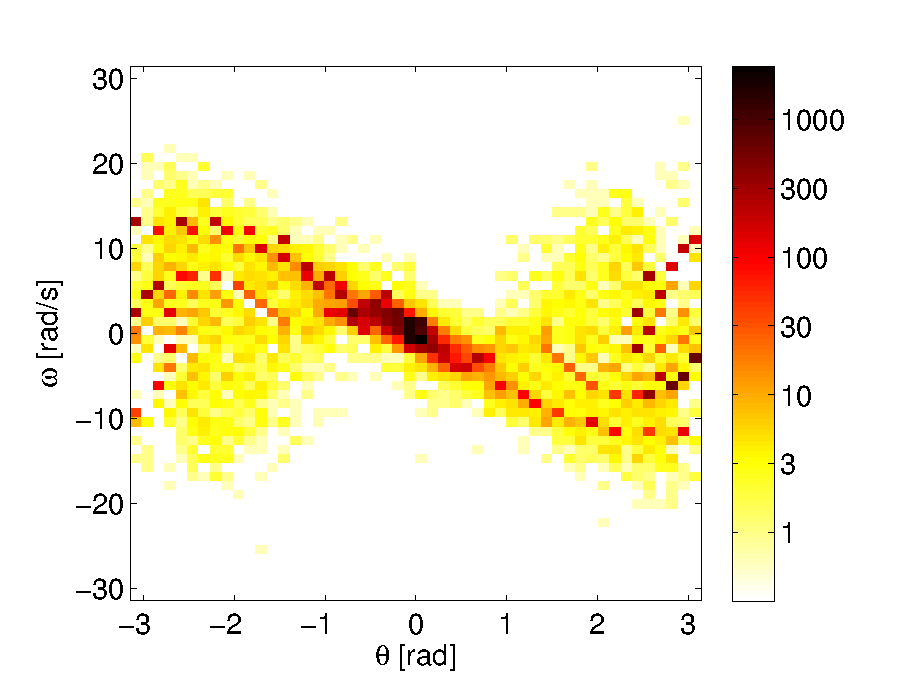
\includegraphics[width=.45\textwidth]{Figures/PS-LA2_hLLR}
	\label{fig:PS-LA2_hLLR}
	}\\
	\subfigure[{$[\delta_\theta,\delta_\omega]=[0.2094,2.0944]$}]{
		\includegraphics[width=.45\textwidth]{Figures/PS-LA3_hLLR}
	\label{fig:PS-LA3_hLLR}
	}
	\subfigure[{$[\delta_\theta,\delta_\omega]=[\infty,\infty]$}]{
		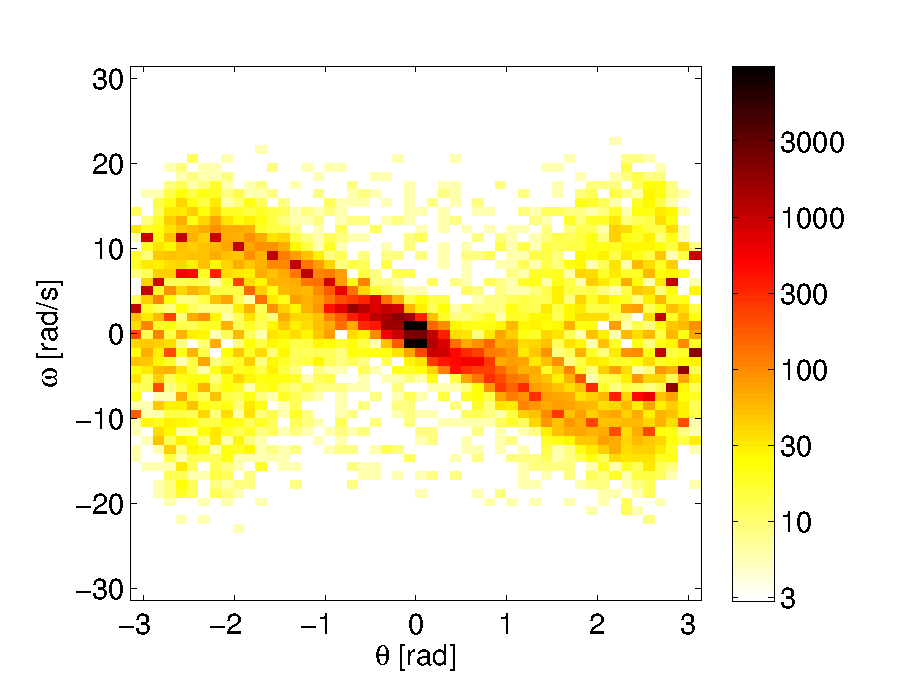
\includegraphics[width=.45\textwidth]{Figures/PS-LA4_hLLR}
	\label{fig:PS-LA4_hLLR}
	} 
	\caption[Inverted pendulum: Distribution of model-generated experience using \acs{LA Dyna}]{Distribution of states for which a state-transition was generated using the \ac{LLR} model in the \ac{LA Dyna} setting. The figures only show the states for which the prediction interval was smaller than the given limit. The color indicates the number of times a state-transition was generated in a certain area.}
	\label{fig:PS-LA_hLLR}
\end{figure}


\section{Conclusions}

In this chapter we have combined model-learning with \acl{RL} to speed up the learning process. We built upon the experience and insight of Chapter \ref{chap:Modeling}. Hence, we used \acl{LLR} as a model. Every experiment was started with an empty memory, which was filled with observed state-transitions during learning. We used an inverted pendulum setup in simulation as experimental setup. A swing-up control task was used to compare different learning algorithms. 

Prediction intervals were used to assess the quality of a modeled state-transition. Whenever the prediction interval of a generated transition is larger than a certain limit, the model output is discarded. We compared four different interval limits, loosely based on the resolution of the value function approximator.

We compared model-free SARSA learning to model-learning Dyna. The Dyna algorithm used state-transitions that were generated randomly throughout the state-space. We showed that the Dyna algorithm performs at least as good as pure SARSA. The Dyna algorithm performed better as more model-generated state-transitions were added. This increased the learning speed and decreased the spread in the curves. Limiting the prediction interval had a negative influence for this setting, as it reduced the number of state-transitions available to the agent. For Dyna the optimal setting would be to use a very loose limit or no limit on the prediction interval at all.

\acl{PS} was combined with \ac{LLR} to determine lead-in state-action pairs. We showed that the limit on the prediction interval is vital for the performance of the \ac{PS} algorithm. Imposing no limit led to very bad performance. In fact, the learning rate was even slower than for SARSA and the algorithm did not converge during a 1000-trial experiment using $[\delta_\theta,\delta_\omega]=[\infty,\infty]$. From the set of four compared prediction intervals, the optimal setting for \ac{PS} was a limit of $[0.2094,2.0944]$. This led to faster learning than the optimal Dyna setting.

Finally, we introduced \acl{LA Dyna} as a learning algorithm. This method uses the \ac{LLR} model to look ahead from the current state. In this way the effect of actions in future states can be assessed. The \ac{LA Dyna} method showed faster learning than the \ac{PS} algorithm. The high number of value-function updates close to the optimal trajectory, makes this method learn fast.
